\documentclass[]{article}

\usepackage{graphicx}
\usepackage{ulem}
\usepackage{xcolor}
\usepackage{clipboard}

%opening
\title{IN2090 2022: Obligatorily assignment 1}
\author{Can Hicabi Tartanoglu}
\date{20th September 2022}

\begin{document}

\maketitle

\section*{Part 1}

\subsection*{Question 1}

There are two entities, Bamle and Ymle. Bamle and Ymle have a relation, Zluff, that is one to many respectively. Every instance of Bamle must have single Zluff relation, and has a unique attribute named Blunk. Zluff is optional for Ymle, it also has the attributes Gru and Blipp; Blipp is unique.

Note that the unique attributes identify each other in the Zluff relation.


\subsection*{Question 2}
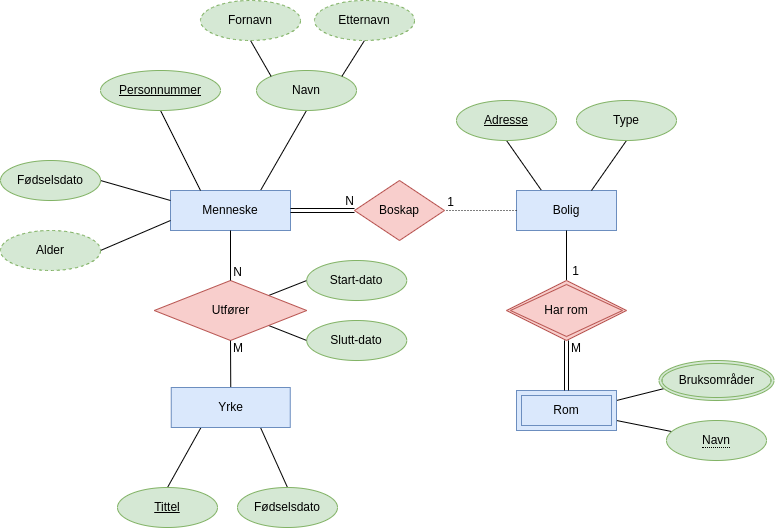
\includegraphics[width=\textwidth]{figures/fig_q2.png}


\section*{Part 2}

\subsection*{Question 3}
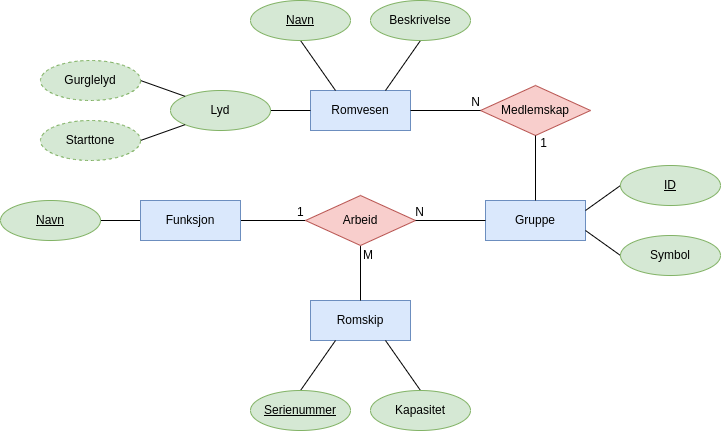
\includegraphics[width=\textwidth]{figures/fig_q3.png}


\subsection*{Question 4}

\subsubsection*{Definitions}

\textbf{PK} = primary key; \textbf{CK} = candidate key; \textbf{FK} = foreign key

\subsubsection*{Answer}

\begin{enumerate}
	\item Mapping regular entity types
		\begin{itemize}
			\item Menneske(\uline{Brukernavn}, \uuline{Personnummer}, MNavn)  where Brukernavn and Personnummer are CKs, I picked Personnumer as PK—it is recognized as an identifier.

			\item \Copy{Melding}{Melding(\uuline{ID}, Diagram, Dato, Klokkeslett)} where ID is the PK.

			\item \Copy{Romvesen}{Romvesen(\uline{RNavn}, Gruppe)}
		\end{itemize}
	
	\item Mapping of weak entity types: \Copy{Vedlegg}{Vedlegg(Innhold, \uline{VNavn, ID})} where ID is the PK of Melding

	\item Mapping of binary 1:N relationship types: I add the PK of Vedlegg, ID, as FK in Menneske: \Copy{Menneske}{Menneske(\uline{Brukernavn}, \uuline{Personnummer}, MNavn, \textcolor{blue}{ID})}

	\item Mapping of binary N:M relationship types: We create a new table to store the relationship, the table stores the PKs of Melding and Romvesen as the composite PK $\rightarrow$ \Copy{M2R}{Medling\_Romvesen(\uline{ID, RNavn})}

	\item Mapping multi-variate attributes: \Copy{M2A}{Menneske\_Ansvarsområde(\uline{Ansvar, Personnummer})} where Personnummer is the FK (the PK of Menneske).
	
\end{enumerate}

\subsubsection*{Result}

\Paste{Menneske}
\\ \\
\Paste{M2A}
\\ \\
\Paste{Melding}
\\ \\
\Paste{Vedlegg}
\\ \\
\Paste{M2R}
\\ \\
\Paste{Romvesen}
\\ \\
\textbf{Foreign keys}
\begin{itemize}
	\item The PK of Melding, \textbf{ID}, is FK in the relation between Melding and Menneske, Vedlegg and Romvesen 
	
	\item The weak attribute key of Vedlegg, \textbf{Navn}, is FK in the Melding relation
	
	\item The PK of Romvesen, \textbf{Navn}, is FK in the Melding reelation
\end{itemize}

\end{document}
